% !TEX root =  master.tex
\section{Startseite mit Filmübersicht}

Auf der Startseite sieht der Benutzer direkt das Kinoprogramm.
Ganz oben befindet sich ein \enquote{Karussell} mit den aktuellen Blockbustern.
Direkt darunter folgt dann die Liste mit den Filmen.

\begin{figure}[ht]
	\centering
	\subfloat[Desktop-Computer]{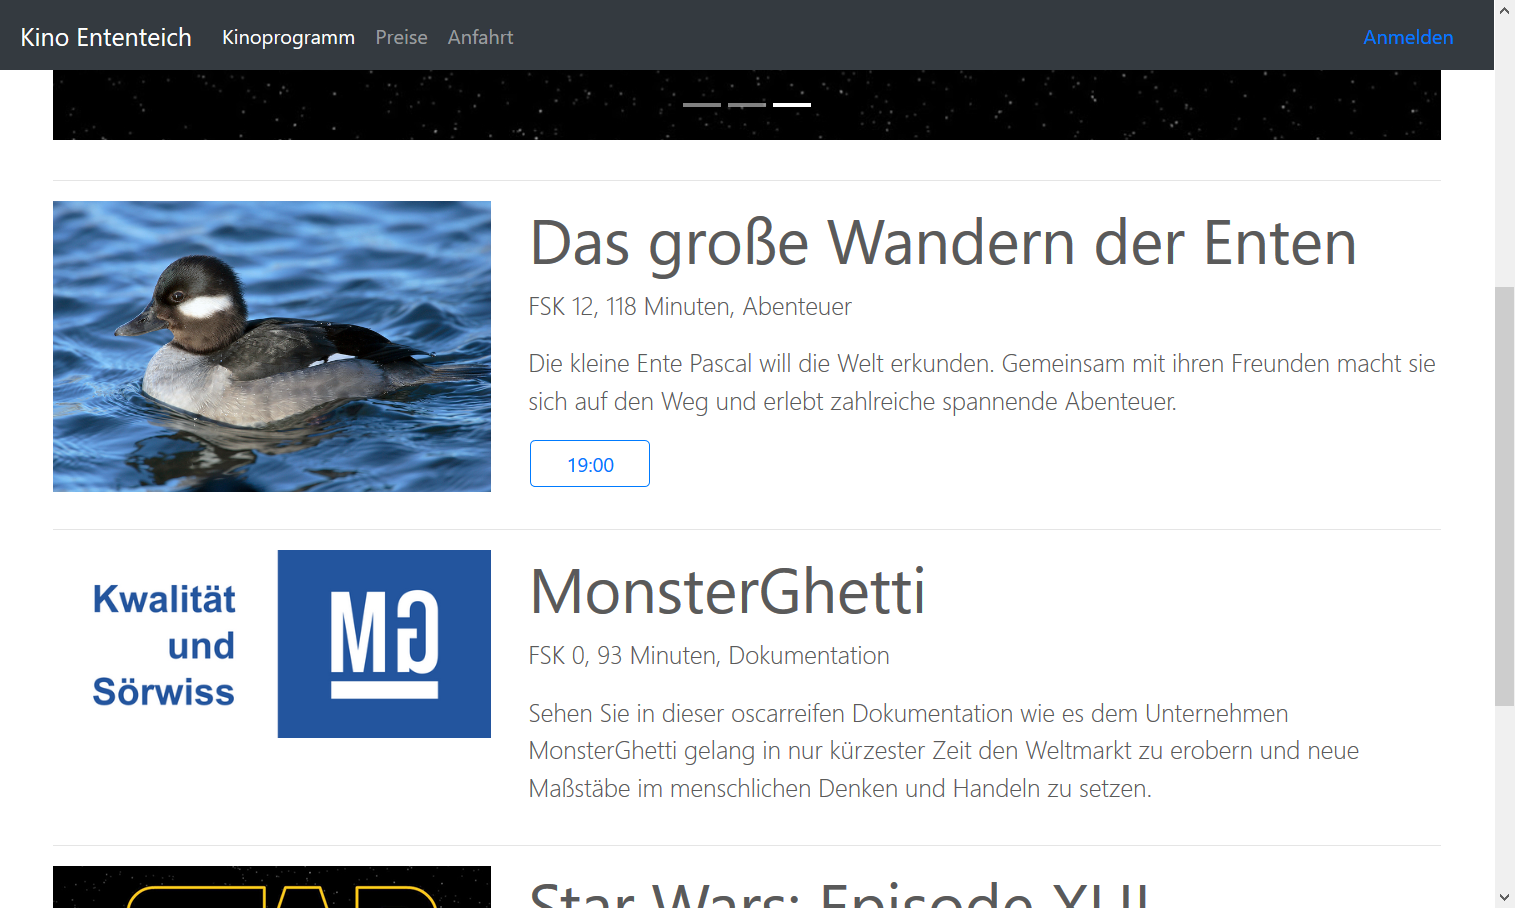
\includegraphics[height=0.28\textheight]{img/screenshots/startseite01}
	\label{fig:startseite01}}
	\hfill
	\subfloat[Mobiles Gerät]{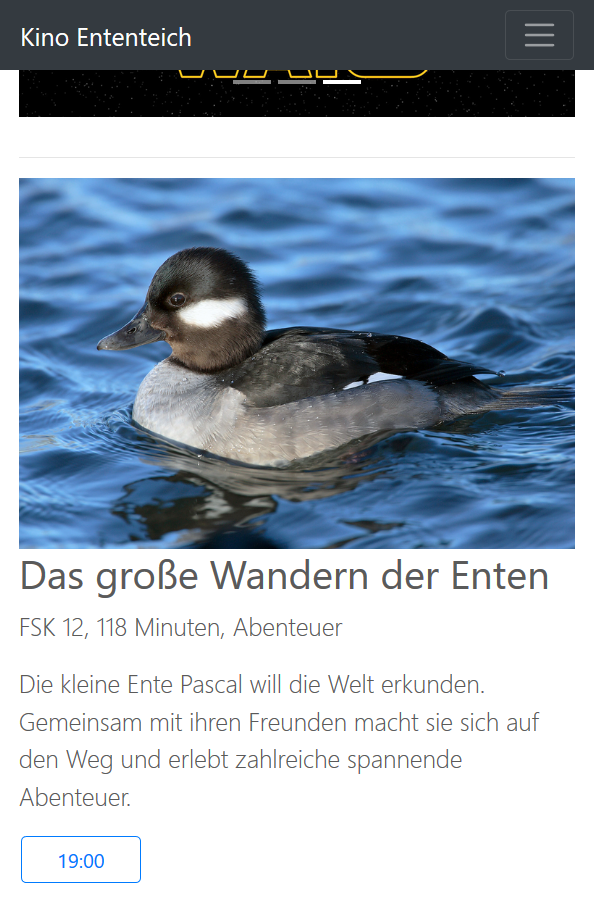
\includegraphics[height=0.28\textheight]{img/screenshots/startseite02}
	\label{fig:startseite02}}
	\caption{Filmübersicht auf der Startseite}
\end{figure}

Dabei ist zu jedem Film neben dem Titel auch noch ein Bild zu sehen.
Allgemeine Informationen zum Film sowie eine Beschreibung ermöglichen es dem Benutzer, sich einen schnellen ersten Eindruck von dem jeweiligen Film zu verschaffen.
Durch Anklicken des Filmtitels oder des Bildes gelangt man zu den Vorstellungen und weiteren Details.
Um Benutzern einen Klick zu ersparen, sieht man sogar direkt die heutigen Vorstellungen und kann gegebenenfalls sofort zu diesen Vorstellungen springen und Sitzplätze auswählen.

Je nach Größe des Bildschirms, wir der Inhalt entsprechend angezeigt.
Bei breiten Bildschirmen, wie es meist bei Desktop-Computern und Laptops der Fall ist, ist genügend Platz, um Bild und Text nebeneinander anzuzeigen.
Bei Smartphones hingegen, wäre das Bild so kaum erkennbar und es würden nicht viele Wörter in eine Zeile passen.
Dementsprechend werden bei solchen Bildschirmen Bild und Text untereinander angezeigt.
All diese Anpassungen werden durch \acs{CSS}-Anweisungen veranlasst, inhaltlich gibt es keine Unterschiede.